\documentclass[15pt,a5paper,reqno]{article}
\usepackage{hyperref}
\usepackage[warn]{mathtext}
\usepackage[utf8]{inputenc}
\usepackage[T2A]{fontenc}
\usepackage[russian]{babel}
\usepackage{amssymb, amsmath, multicol}
\usepackage{graphicx}
\usepackage[shortcuts,cyremdash]{extdash}
\usepackage{wrapfig}
\usepackage{floatflt}
\usepackage{lipsum}
\usepackage{verbatim}
\usepackage{concmath}
\usepackage{euler}
\usepackage{xcolor}
\usepackage{etoolbox}
\usepackage{fancyhdr}
\usepackage{subfiles}
\usepackage{enumitem}
\usepackage{amsthm}
\usepackage{indentfirst}
\usepackage{import}

\DeclareMathOperator{\sign}{sign}

\RequirePackage[ left     = 1.5cm,
  right    = 1.5cm,
  top      = 2.0cm,
  bottom   = 1.25cm,
  includefoot,
  footskip = 1.25cm ]{geometry}
\setlength    {\parskip}        { .5em plus .15em minus .08em }
%\setlength    {\parindent}      { .0em }
\renewcommand {\baselinestretch}{ 1.07 }

\fancyhf{}

\renewcommand{\footrulewidth}{ .0em }
\fancyfoot[C]{\texttt{\textemdash~\thepage~\textemdash}}
\fancyhead[R]{\hfilШурыгин}

\makeatletter
\patchcmd\l@section{%
  \nobreak\hfil\nobreak
}{%
  \nobreak
  \leaders\hbox{%
    $\m@th \mkern \@dotsep mu\hbox{.}\mkern \@dotsep mu$%
  }%
  \hfill
  \nobreak
}{}{\errmessage{\noexpand\l@section could not be patched}}
\makeatother
\parindent = 1cm % отступ при красной строке⏎
\pagestyle{fancy}    
\renewcommand\qedsymbol{$\blacksquare$}

\newcommand{\when}[2]{
  \left. #1 \right|_{#2} \hspace
}
\renewcommand{\kappa}{\varkappa}
\RequirePackage{caption2}
\renewcommand\captionlabeldelim{}
\newcommand*{\hm}[1]{#1\nobreak\discretionary{}

\DeclareSymbolFont{T2Aletters}{T2A}{cmr}{m}{it}
{\hbox{$\mathsurround=0pt #1$}}{}}
% Цвета для гиперссылок
\definecolor{linkcolor}{HTML}{000000} % цвет ссылок
\definecolor{urlcolor}{HTML}{799B03} % цвет гиперссылок
 
\hypersetup{pdfstartview=FitH,  linkcolor=linkcolor,urlcolor=urlcolor, colorlinks=true}


\begin{document}

	% НАЧАЛО ТИТУЛЬНОГО ЛИСТА

\begin{titlepage}
	\begin{center}
		\large 	Московский физико-технический университет \\
		Физтех-школа радиотехники и компьютерных технологий\\
		\vspace{0.2cm}
		
		\vspace{4.5cm}
		Лабораторная работа № 3.2.2 \\ \vspace{0.2cm}
		\LARGE \textbf{Резонанс напряжения в электрическом контуре}
	\end{center}
	\vspace{2.3cm} \large
	
	\begin{center}
		Работу выполнил: \\
		Шурыгин Антон \\
		Б01-909

	\end{center}
	
	\begin{center} \vspace{60mm}
		г. Долгопрудный \\
	\end{center}
\end{titlepage}


	\textbf{Цель работы:} исследовать сериальные закономерости в оптическом спектре водорода; спектр поглощения паров йода в видимой области.
	
    \section{Введение и краткая теория}

    В работе предлагается измерить фокусные расстояния линз, смоделировать трубу Кеплера, трубу Галилея
    микроскоп и определить их увеличения.
    \newline

    \textbf{Сложенин центрированных оптических систем}
    Пусть две центрированные системы имеют общую главную оптическую ось. Если известны параметры каждой системы, а также их взаимное расположение, то аналитическим расчётом или геометрическим
    построением можно определить положение всех кардинальных точек
    сложной оптической системы, состоящей из этих двух систем.

    Рассматриваемая система схематически изображена на рис. 1.3.
    Кардинальные точки первой и второй систем отмечены соответствующими нижними индексами. Штрихами выделены кардинальные точки
    пространства изображений первой системы и аналогичные точки пространства предметов второй системы. 
    Величина $\Delta = F2 - F'1$ представляет расстояние от заднего фокуса первой системы до переднего фокуса
    второй системы и называется оптическим интервалом двух систем. 
    В соответствии с принятым правилом знаков $\Delta > 0$, если падающий светидёт от фокуса $F'1$ к фокусу $F2$, как отмечено стрелкой на рис. 1.3, в
    противоположном случае $\Delta < 0$. Заданием оптического интервала полностью определяется взаимное расположение складываемых систем.

    \begin{figure}[h!]
        \centering
        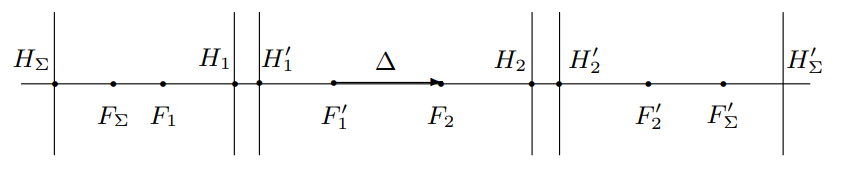
\includegraphics[width=0.8\linewidth]{pics/system_of_lens.png}
        \caption{Сложение центрированных систем}
        \label{}
    \end{figure}


    Конечные уравнения для фокусного расстояния и координат фокальных и главных точек сложной системы:


    \begin{equation}\label{1}
        f_{\sum} = - \frac{f_1 f_2}{\Delta}
    \end{equation}


    \begin{equation}\label{2}
        f'_{\sum } = - \frac{f'_1 f'_2}{\Delta}
    \end{equation}

    \begin{equation}\label{3}
        \Phi = \frac{n}{f_{\sum}} = -\frac{n\Delta}{f_1 f_2}
    \end{equation}



    \textbf{Примеры центрированных оптических систем}
    Оптическая система может не иметь фокальных плоскостей. Такая система называется афокальной или телескопической.
    Она является предельным случаем обычной системы, у которой фокальные плоскости сдвинуты в беконечность.
    Как видно из формул для сложных систем, телескопической становится система из двух обычных систем, если их оптический интервал $\Delta \rightarrow 0$

    Выполнив этот предельный переход в уравнениях, получим формулы для преобразования координат и коэффициенты увеличений телескопической системы:

    \[ \frac{x'}{x} = \frac{\delta x'}{\delta x} = \frac{f_2 f'_2}{f_1 f'_1} \]
    \[ \frac{y'}{y} = \frac{n \alpha}{n' \alpha'} = \frac{f_2}{f'_1} \]
    

    Из выражений выше следует, что в телескопической системе:
    \begin{enumerate}
        \item всякий параллельный пучок света после прохождения через систему остаётся параллельным
        \item продольное, поперечное и угловое увеличения постоянны, то есть не зависят от положения предмета.
    \end{enumerate}

    Оптическая сила телескопической системы, как видно из формулы \ref{3}, равна нулю.

       
        \section{Экспериментальная установка}
        Для измерения длин волн спектральных линий в работе используется стеклянный-призменный монохроматор-спектрометр УМ-2, предназначенный для спектральных исследований.
        

        \begin{figure}[h!]
            \centering
            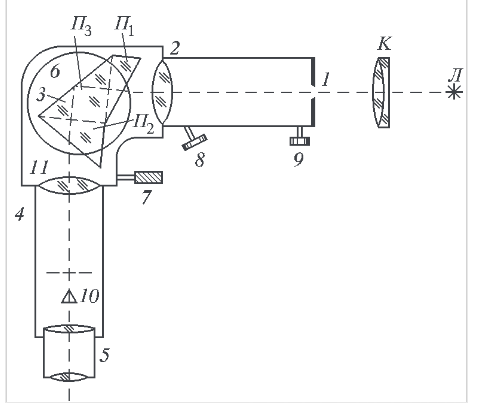
\includegraphics[width=0.8\linewidth]{pics/scheme1.png}
            \caption{Устройство монохроматора УМ-2}
            \label{scheme1}
        \end{figure} 
        
        В работе спектр поглощения паров йода наблюдается визуально на фоне сплошного спектра лампы накаливания, питаемой от блока питания.
        
        
        \begin{figure}[h!]
            \centering
            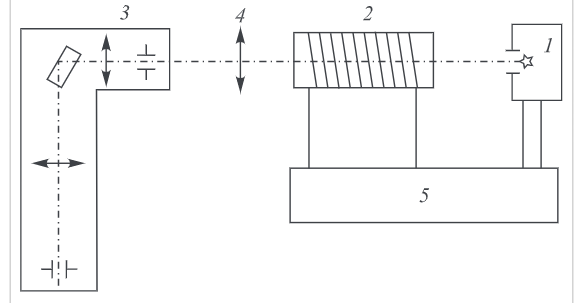
\includegraphics[width=0.8\linewidth]{pics/scheme2.png}
            \caption{Схема экспериментальной установки для изучения спектра поглощения паров йода}
            \label{scheme2}
        \end{figure} 
        
        \newpage

        \section{Ход работы и обработка данных}
        
        Калибровка спектрометра была выполнена по спектрам ртути и неона. По ртути следует калиброваться в коротковолновой части спектра, а по неону -- в средней и длинноволновой.

        \begin{table}[h!]
            \centering
            \begin{tabular}{| c | c | c | c | c |}
\hline
$U, mV$ & $T_{room}, K$ & $T, K$ & $T_{br}, K$ & $ \sigma_{T}, K$\\
\hline
$39920$ & $298$ & $973,66$ & $1000$ & $ 28 $\\
\hline
\end{tabular}

            \caption{: калибровка для неона}
        \label{tb1}
        \end{table}
    
        \begin{table}[h!]
            \centering
            \begin{tabular}{| c | c | c | c | c |}
\hline
$\theta,^{\circ}$ & $U(I)$ & $V_{ФЭ}$ & $\sigma_{U(I)}$ & $\sigma_{V_{ФЭ}}$\\
\hline
$2404$ & $0,036$ & $0,302$ & $0,0004$ & $0,003$\\
\hline
$$ & $0,032$ & $0,262$ & $0,0004$ & $0,003$\\
\hline
$$ & $0,027$ & $0,202$ & $0,0004$ & $0,003$\\
\hline
$$ & $0,02$ & $0,121$ & $0,0004$ & $0,003$\\
\hline
$$ & $0,016$ & $0,039$ & $0,0004$ & $0,003$\\
\hline
$$ & $0,009$ & $-0,062$ & $0,0004$ & $0,003$\\
\hline
$$ & $0,006$ & $-0,162$ & $0,0004$ & $0,003$\\
\hline
$$ & $0$ & $-0,303$ & $0,0004$ & $0,003$\\
\hline
\end{tabular}

            \caption{: калибровка для ртути}
        \label{tb2}
        \end{table}

		Проградуируем спектрометр, для чего используем спектры неоновой и ртутной лампы, длины волн спектральных линий которых известны. 
		
        \begin{figure}[h!]
            \centering
            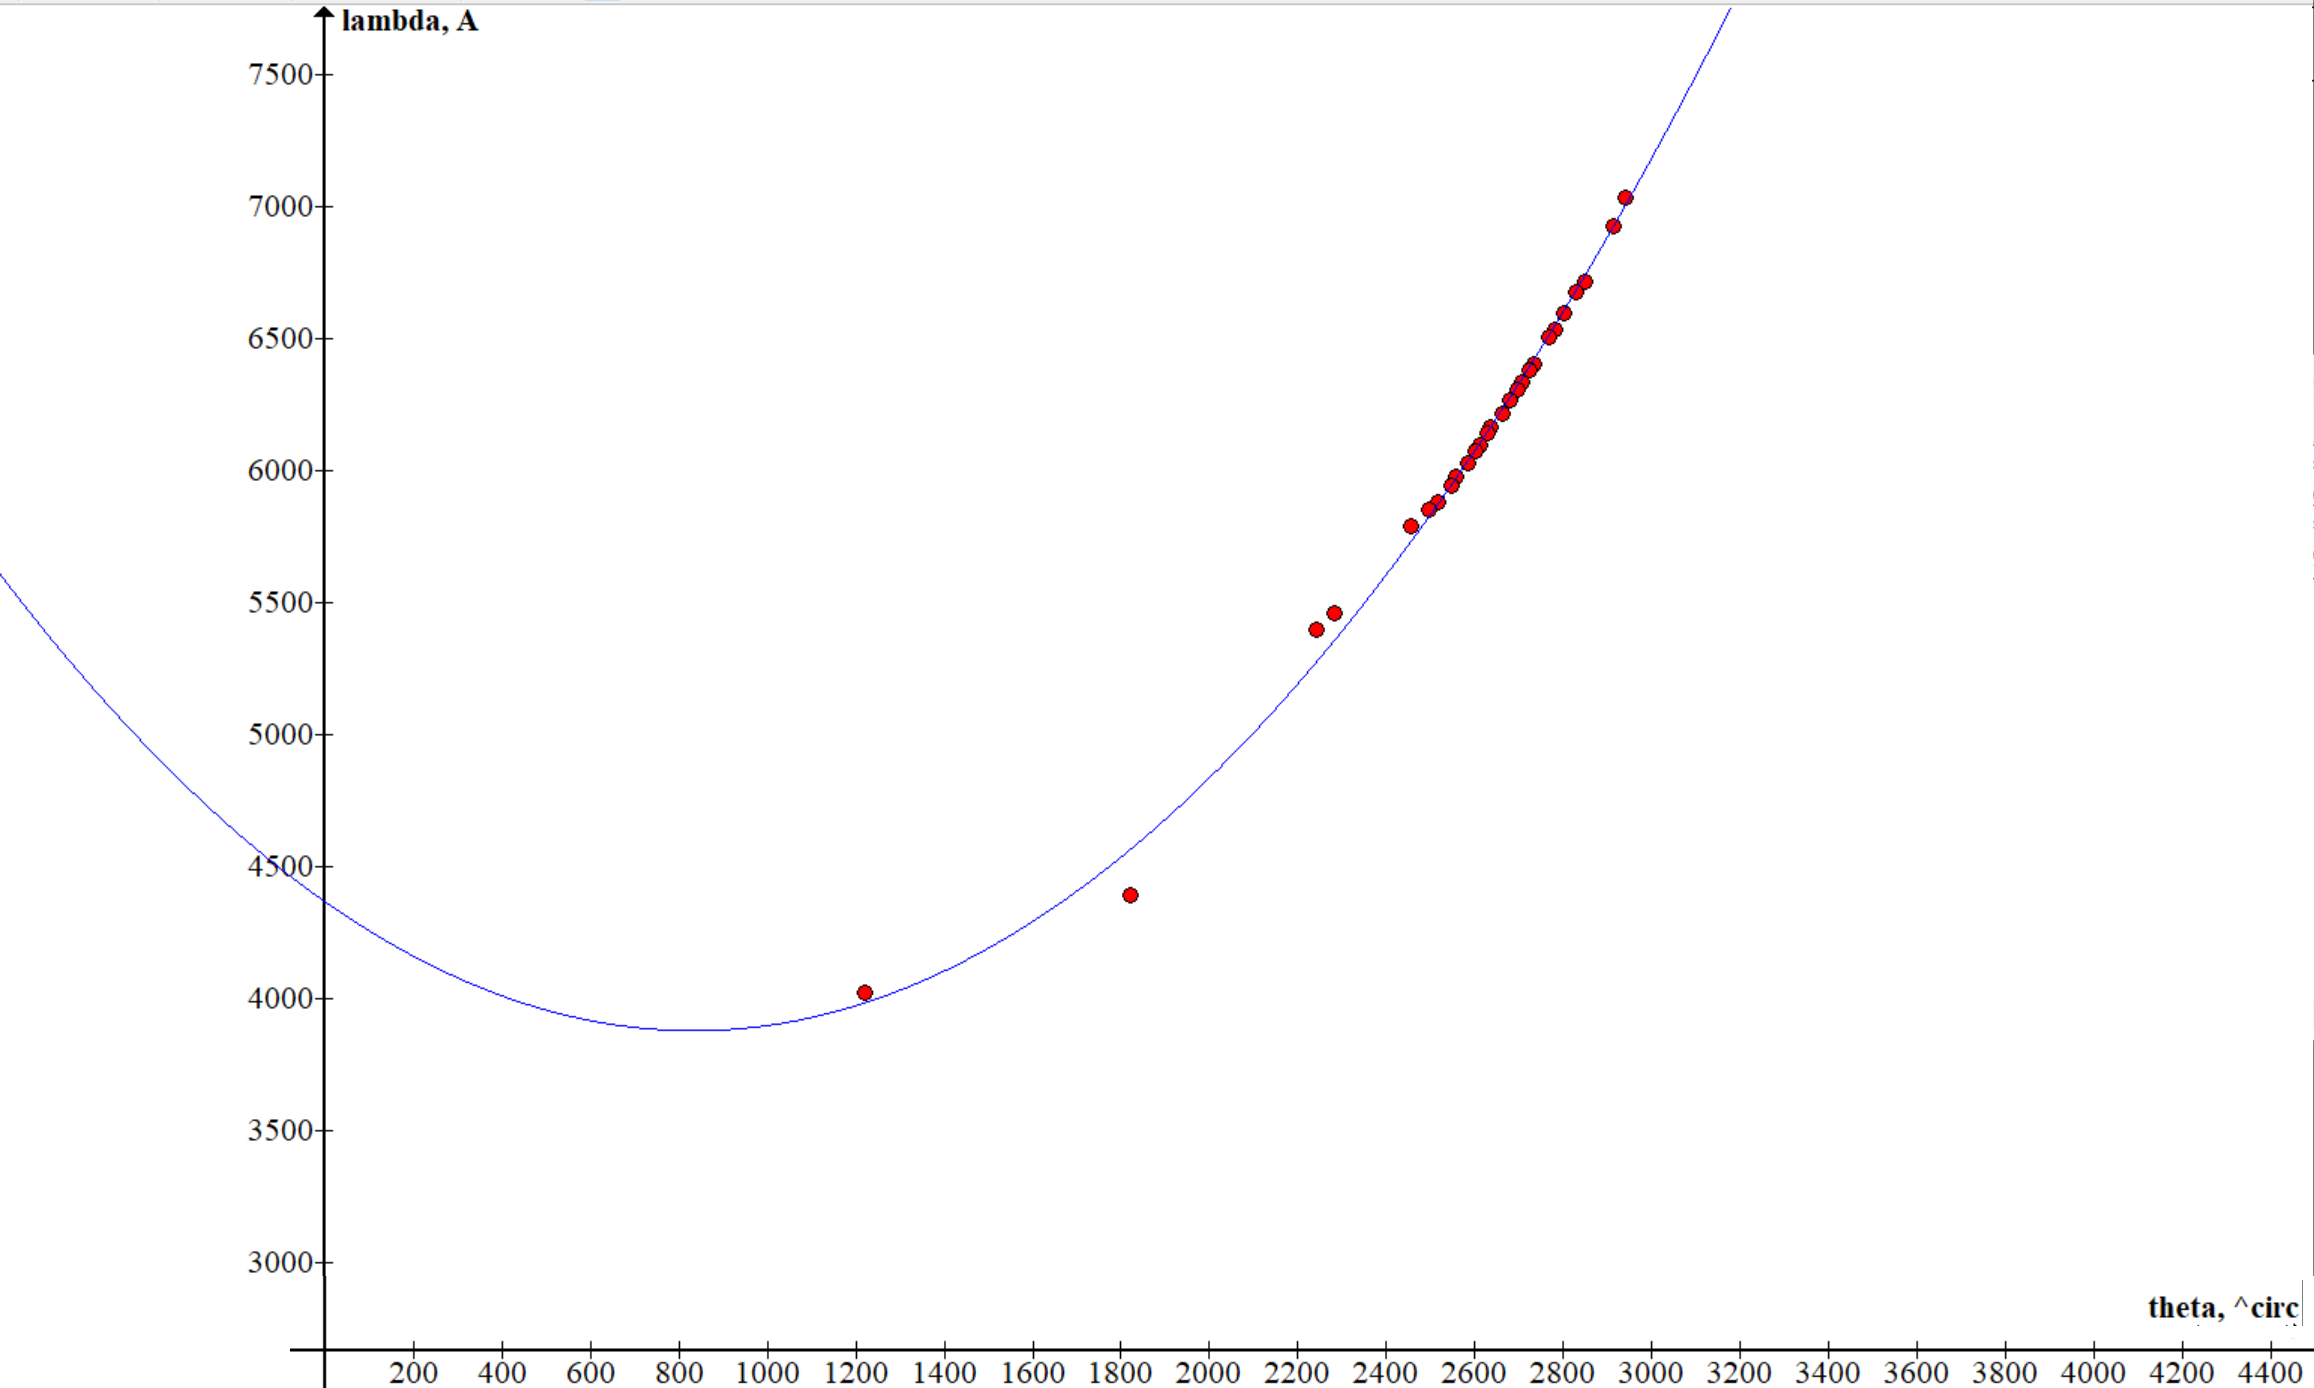
\includegraphics[width=1.0\linewidth]{pics/grad.png}
            \caption{ : градуировка спектрометра}
            \label{al}
        \end{figure}
	
        Получаем приближение полиноном второй степени: 
        
        \[ f(x) = 0,00007x^{2} -1,1725x + 4369,6081 \]

		Измерим положения трёх линий водорода из серии Бальмера --- $H_{\alpha}, H_{\beta}, H_{\gamma}$. Линии $H_{\delta}$ и более коротковолновые пронаблюдать не удалось ввиду их слабой интенсивности.	Получили соответствующие показания спектрометра:
		\begin{equation*}
			H_{\alpha}: (2792\pm 5), \  H_{\beta} : (1814 \pm 5), \ H_{\gamma} : (1172 \pm 5).
		\end{equation*}
		С учётом градуировки спектрометра получаем следующие длины волн: 
		\begin{equation*}
			H_{\alpha} = (650\pm 20)\ \text{нм}, \ H_{\beta} = (487\pm 15)\ \text{нм}, \ H_{\gamma} = (430\pm  20)\  \text{нм}.
		\end{equation*}
		
		
		Для каждой линии определим константу Ридберга по формуле (\ref{eq:Ry}), учитывая, что $m=2$, $Z=1$, а также, что для линии $H_{\alpha}$ --- $n=3$, для линии $H_{\beta}$ --- $n=4$, для линии $H_{\gamma}$ --- $n=5$. Получаем следующие значения константы Ридберга:
		\begin{equation*}
			\text{Ry}_{\alpha}=(1.114\pm 0.05) \cdot 10^{-2} \ \text{нм}^{-1}, \ \text{Ry}_{\beta} =(1.10\pm 0.05)\cdot 10^{-2} \ \text{нм}^{-1}, \ \text{Ry}_{\gamma}=(1.11\pm 0.05)\cdot 10^{-2}\ \text{нм}^{-1}.
		\end{equation*}
	
		Возьмем среднее среди полученных значений константы Ридберга и определим её экспериментально полученное значение:
		
		\[ \text{Ry}_E=(1.105\pm 0.05)\cdot 10^{-2} ~\text{нм}^{-1} \]
		Полученное значение вполне неплохо совпадает с табличным значением: 
		\[ \text{Ry}=1.097\cdot 10^{-2} \ \text{нм}^{-1} \]
		
		Запишем показания спектрометра для следующих переходов в молекуле йода: $\theta_{1,0}$ -- переход из первого колебательного уровня основного состояния в нулевой колебательный уровень возбуждённого состояния,  $\theta_{1,5}$ -- переход из первого колебательного уровня основного состояния в пятый колебательный уровень возбуждённого состояния, $\theta_{g}$ -- переход из нулевого колебательного уровня основного состояния в область непрерывного спектра возбуждённого состояния. Получаем следующие данные:
		\begin{equation*}
			\theta_{1,0}=(2700\pm 15), \ \theta_{1,5}=(2620\pm 20), \ \theta_g=(2000\pm 20),
		\end{equation*}
		 откуда находим соответствующие длины волн: 
		 
		 \begin{equation*}
		 	\lambda_{1,0}=(620\pm 30) \ \text{нм}, \ \lambda_{1,5}=(610\pm 30) \ \text{нм}, \ \lambda_g=(510\pm 30)\ \text{нм}.
		 \end{equation*}
		
		Определим энергию колебательного кванта возбуждённого состояния молекулы по формуле: 
		\begin{equation*}
			h \nu_2=\dfrac{h\nu_{1,5}-h \nu_{0,5}}{5}.
		\end{equation*}
		Итого:
		\begin{equation*}
			h\nu_2=(1.0\pm 0.2)\cdot 10^{-2} \ \text{эВ}
		\end{equation*}
			
		Вычислим энергию электронного перехода $\Delta E=E_2-E_1$, энергию диссоциации $D_1$ в основном состоянии и энергию диссоциации $D_2$ в возбуждённом состоянии, если известно, что энергия колебательного кванта основного состояния есть $h\nu_1=0,027$~эВ, а энергия возбуждения, то есть энергия перехода атома из области непрерывного спектра основного состояния в область непрерывного спектра возбуждённого состояния, равна $E_A=0.94$ эВ.\\
		Имеем систему уравнений:
		\begin{equation*}
			\begin{cases}
				D_1+E_A=h \nu_g,\\
				h\nu_g=D_2+\Delta E,\\
				h\nu_{1,0}=\Delta E+h\nu_2-\dfrac{3}{2}h\nu_1,\\
					h\nu_{1,5}=\Delta E+\dfrac{11}{2}h\nu_2-\dfrac{3}{2}h\nu_1.
			\end{cases}
		\end{equation*}

		Из неё находим все необходимые величины:
		\[ \Delta E=(2.0\pm 0.1) \ \text{эВ}, \ D_1=(1.5\pm 0.1)\  \text{эВ}, \  D_2=(0.42\pm 0.08) \ \text{эВ} \]

\section{Вывод}
	В работе исследовались сериальные закономерности в оптическом спектре водорода и спектр поглощения паров йода в видимой области.
	
	Получены длины волн линий $H_{\alpha}$, $H_{\beta}$ и $H_{\gamma}$ серии Бальмера, вычислена постоянная Ридберга. 
    
    \[ \text{Ry}_E=(1.105\pm 0.05)\cdot 10^{-2} ~\text{нм}^{-1} \]
	
	Получены длины волн, соответствующие некоторым электронно-колебательным переходам из основного состояния в возбуждённое. Вычислены энергия колебательного кванта возбуждённого состояния молекулы, энергия электронного перехода, энергии диссоциации молекулы в основном и в возбуждённом состояниях.
	$h\nu_2=(1.0\pm 0.2)\cdot 10^{-2} \ \text{эВ}$


\end{document}